\chapter[Implementación]{
  \label{chp:implementacion}
  IMPLEMENTACIÓN
}
\thispagestyle{numberingStyle}
\pagestyle{numberingStyle}



\section{Estructura de la aplicación}
\subsection{Estructura proyecto Java}
Para la implementación del modelo y la aplicación web, se ha elaborado un proyecto Maven con los siguientes módulos:
\\
\\

\begin{figure}[H]
\centering
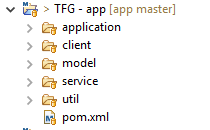
\includegraphics[
   keepaspectratio=true
]{./06_Implementacion/img/estructuraglobaljava.png}
\caption{Estructura proyecto Java}
\end{figure}


\begin{itemize}
	\item \textbf{TFG - app: } Es el proyecto Maven de la aplicación Java. Está formado por diferentes módulos que forman la aplicación:
	\begin{itemize}
		\item \textbf{Application: } Es un módulo donde se encuentran las aplicaciones web del sistema.
		\item \textbf{Client: } Es un módulo donde se implementa el cliente que consume y accede los servicios del modelo. Necesario para la aplicación web.
		\item \textbf{Model: } Donde reside la persistencia y la lógica de negocio de la aplicación.
		\item \textbf{Service : } Es el módulo que define e implementa los servicios.
		\item \textbf{Util : } Módulo de utilidad. Aporta clases y funciones comunes a los demás módulos.
		\item \textbf{pom.xml : } Archivo utilizado por Maven para la construcción del proyecto, manteniendo la gestión de las dependencias y el orden de construcción de los módulos.
	\end{itemize}
\end{itemize}

Con esta separación en módulos conseguimos hacer más independiente cada uno de los módulos que formarán el desplegable de la aplicación. De tal manera, que si queremos utilizar otra implementación de persistencia, simplemente tenemos que reemplazar el JAR generado por dicho módulo por el que queramos utilizar, en el archivo de aplicación web (WAR).

\subsubsection*{Módulo Model}
El módulo \textit{model} de la aplicación está compuesto por: \textit{core} y \textit{persistence}.

\begin{figure}[H]
\centering
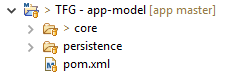
\includegraphics[
   keepaspectratio=true
]{./06_Implementacion/img/estructuramodeljava.png}
\caption{Estructura módulo \textit{model}}
\end{figure}

En el submódulo \textit{persistence} se implementa toda la persistencia de datos, desde las clases persistentes hasta las definiciones e implementaciones de los DAOs. Por su parte, en el submódulo \textit{core} se define e implementa la lógica de negocio.

\subsubsection*{Estructura directorios Model - Persistence}
\begin{figure}[H]
\centering
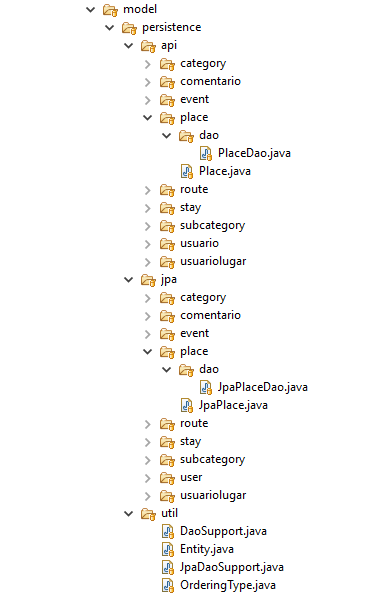
\includegraphics[
   keepaspectratio=true
]{./06_Implementacion/img/estructuramodelpersistence.png}
\caption{Estructura módulo \textit{model-persistence}}
\end{figure}

\begin{itemize}
	\item \textbf{src/main/java/ ../model/persistence/api. } Es el directorio donde se encuentran todas las definiciones de las clases persistentes (Ej: Place.java) y los DAOs (Ej: PlaceDao.java).
	\item \textbf{src/main/java/ ../model/persistence/jpa. } Directorio donde residen las implementaciones de las definiciones anteriores (Ej: JpaPlace.java, JpaPlaceDao.java). Como su nombre indica, se hace uso del API de persistencia JPA. 
	\item \textbf{src/main/java/ ../model/persistence/util. } Es el directorio donde se incluyen clases de utilidad (Ej: DaoSupport y JpaDapSupport, para la implementación de los DAOs).
\end{itemize}

\subsubsection*{Estructura directorios Model - Core}
\begin{figure}[H]
\centering
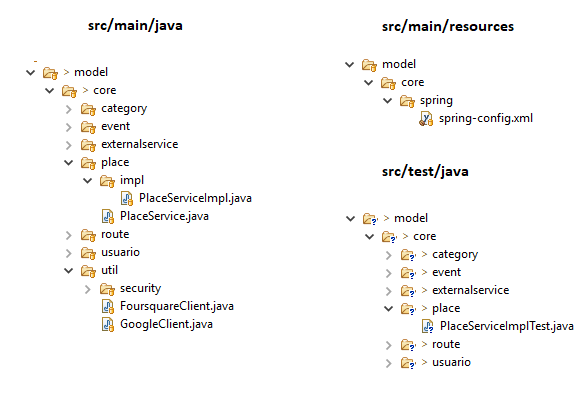
\includegraphics[
   keepaspectratio=true
]{./06_Implementacion/img/estructuramodelcore.png}
\caption{Estructura módulo \textit{model-core}}
\end{figure}

\begin{itemize}
	\item \textbf{src/main/java/ ../model/core. } Directorio donde se especifican e implementan la lógica de negocio de la aplicación.
	\item \textbf{src/main/java/ ../model/core/util. } Directorio de utilidad que incluye los clientes de las APIs externas.
	\item \textbf{src/test/java/ ../model/core. } Incluye las pruebas automatizadas para cada uno de lo servicios de la lógica de negocio.
\end{itemize}


\subsubsection*{Módulo Service}
El módulo \textit{service} de la aplicación está compuesto por los submódulos \textit{api} y \textit{core}.

\begin{figure}[H]
\centering
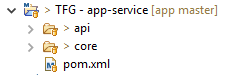
\includegraphics[
   keepaspectratio=true
]{./06_Implementacion/img/estructuraservice.png}
\caption{Estructura módulo \textit{service}}
\end{figure}


\subsubsection*{Estructura directorios Service - Api}
\begin{figure}[H]
\centering
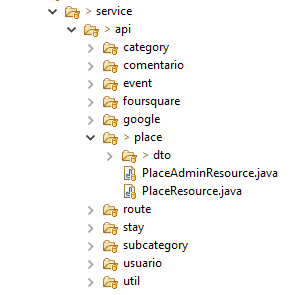
\includegraphics[
   keepaspectratio=true
]{./06_Implementacion/img/estructuraserviceapi.png}
\caption{Estructura módulo \textit{service-api}}
\end{figure}

\begin{itemize}
	\item \textbf{src/main/java/ ../service/api. } Directorio donde se definen cada uno de los recursos web, siguiendo la API de JAX-RS que ofrece el soporte para la creación de servicios web, que ofrecerán remotamente, los servicios de la capa modelo. Se puede observar la definición dos recursos web, como son: \textit{PlaceResource.java} y \textit{PlaceAdminResource.java}.
\end{itemize}


\subsubsection*{Estructura directorios Service - Core}
\begin{figure}[H]
\centering
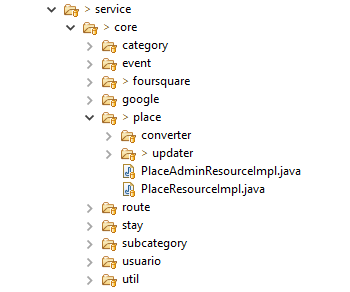
\includegraphics[
   keepaspectratio=true
]{./06_Implementacion/img/estructuraservicecore.png}
\caption{Estructura módulo \textit{service-core}}
\end{figure}

\begin{itemize}
	\item \textbf{src/main/java/ ../service/core. } Directorio con las implementaciones para cada uno de los recursos definidos en el submódulo \textit{service-api}. Se puede observar las clases \textit{PlaceResourceImpl.java} y \textit{PlaceAdminResourceImpl.java} que implementa las clases mostradas en el submódulo anterior.
	\begin{itemize}
		\item \textbf{../service/core/*/converter. } Directorio con las clases necesarias para la conversión de objetos a persistentes a objetos de transferencia de datos.
		\item \textbf{../service/core/*/updater. } Directorio con las clases necesarias para la creación del objeto persistente a modificar a partir del objeto de transferencia de datos recibido. 
		\item \textbf{../service/core/util. } Directorio en el que se encuentran clases que ofrecen funcionalidades como la conversión de excepciones Java a respuestas HTTP, validadores de datos de entrada, etc...
	\end{itemize}
\end{itemize}



\subsubsection*{Módulo Application}
\begin{figure}[H]
\centering
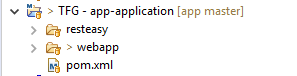
\includegraphics[
   keepaspectratio=true
]{./06_Implementacion/img/estructuraapplication.png}
\caption{Estructura módulo \textit{application}}
\end{figure}

Formado por los submódulos \textit{resteasy} y \textit{webapp}. El primero de ellos será el encargado de ofrecer una aplicación REST, donde se expondrán remotamente, los servicios creados en la capa de servicios del modelo. Utilizará el proyecto \textit{JBoss RESTEasy} como implementación del API de JAX-RS.

Por su parte, el módulo \textit{webapp} será el encargado de ofrecer una aplicación web, accesible mediante navegador web. Seguirá una arquitectura MVC.


\subsubsection*{Estructura directorios Application - Resteasy}
\begin{figure}[H]
\centering
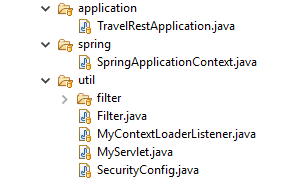
\includegraphics[
   keepaspectratio=true
]{./06_Implementacion/img/estructuraapplicationresteasy.png}
\caption{Estructura módulo \textit{application-resteasy}}
\end{figure}

\begin{itemize}
	\item \textbf{src/main/java/ ../application/resteasy. }
	\begin{itemize}
		\item \textbf{../application/resteasy/application. } Directorio con la clase encargada de añadir al contenedor de la aplicación los objetos definidos en la capa de servicios.		
		\item \textbf{../application/resteasy/filter. } Directorio en el que se encuentran los filtros de la aplicación.
		\item \textbf{../application/resteasy/spring. } Directorio con la clase encargada de obtener los objetos del contenedor de Spring y poder incorporarlos al contenedor de la aplicación. para su uso.
	\end{itemize}
\end{itemize}



\subsubsection*{Estructura directorios Application - Webapp}
\begin{figure}[H]
\centering
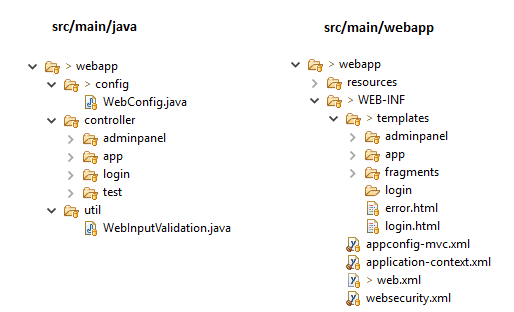
\includegraphics[
   keepaspectratio=true
]{./06_Implementacion/img/estructuraapplicationwebapp.png}
\caption{Estructura módulo \textit{application-resteasy}}
\end{figure}

\begin{itemize}
	\item \textbf{src/main/java. }
	\begin{itemize}
		\item \textbf{../application/webapp/config. } Directorio donde residen archivos de configuración de la aplicación.
		\item \textbf{../application/webapp/controller. } Directorio en el que se encuentran implementados los controladores de la aplicación.
		\item \textbf{../application/webapp/util. } Directorio con las clases de utilidad.
	\end{itemize}
	\item \textbf{src/main/webapp. }
	\begin{itemize}
		\item \textbf{../application/webapp/resources. } Directorio con los ficheros que aportan un mejor aspecto a la web. Incluye, archivos JavaScript, CSS e imágenes.
		\item \textbf{../application/webapp/WEB-INF. } Directorio en el que se encuentran las plantillas HTML utilizadas para crear las páginas web.
	\end{itemize}
\end{itemize}


\subsubsection*{Módulo Client}
\begin{figure}[H]
\centering
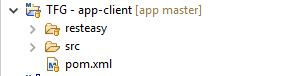
\includegraphics[
   keepaspectratio=true
]{./06_Implementacion/img/estructuraclient.png}
\caption{Estructura módulo \textit{client}}
\end{figure}

El módulo \textit{client} está compuesto, únicamente, del módulo \textit{resteasy}. Este módulo, define e implementa un cliente para la aplicación REST anteriormente comentada.


\subsubsection*{Estructura directorios Client - Resteasy}
\begin{figure}[H]
\centering
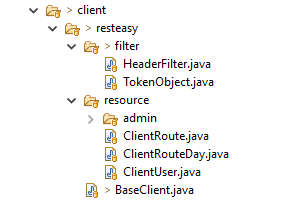
\includegraphics[
   keepaspectratio=true
]{./06_Implementacion/img/estructuraclientresteasy.png}
\caption{Estructura módulo \textit{client-resteasy}}
\end{figure}

\begin{itemize}
	\item \textbf{src/main/java/ ../client/resteasy. }
	\begin{itemize}
		\item \textbf{../resteasy/filter. } Directorio donde residen los filtros utilizados por el cliente.
		\item \textbf{../resteasy/resource. } Directorio en el que se encuentran implementados los clientes específicos para cada servicio.
	\end{itemize}
\end{itemize}

\newpage
\subsection{Estructura proyecto Ionic}
Ionic presenta una estructura típica de proyecto Cordova donde se pueden instalar complementos nativos y crear archivos de proyecto, específicos para cada plataforma. La estructura con los ficheros de código fuente es la siguiente:

\begin{figure}[H]
\centering
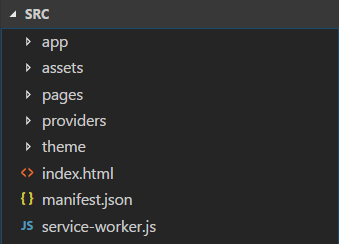
\includegraphics[
   keepaspectratio=true
]{./06_Implementacion/img/estructuraionicsrc.png}
\caption{Estructura aplicación \textit{Ionic}}
\end{figure}

\begin{itemize}
	\item \textbf{src/index.html. } Punto de entrada de la aplicación que tiene como propósito la configuración de \textit{scripts} y hojas de estilo para arrancar la aplicación.
	\item \textbf{src/app. } Directorio con las clases que inician la aplicación.
	\item \textbf{src/assets. } Directorio que almacena recursos de estáticos, como imágenes, iconos, etc...
	\item \textbf{src/pages. } Directorio en el que se encuentran las diferentes vistas y controladores que forman la aplicación.
	\item \textbf{src/providers. } Directorio que incluye las clases que implementan el acceso a los servicios y clases que implementan determinadas funcionalidades en la aplicación.
	\item \textbf{src/theme. } Directorio con las clases SASS que especifican ciertos aspectos de estilo de la aplicación.
\end{itemize}


\subsubsection*{Estructura directorio pages}
En la siguiente figura, se muestra el subdirectorio \textit{pages}, que incluye todas las vistas y controladores de la aplicación.
\begin{figure}[H]
\centering

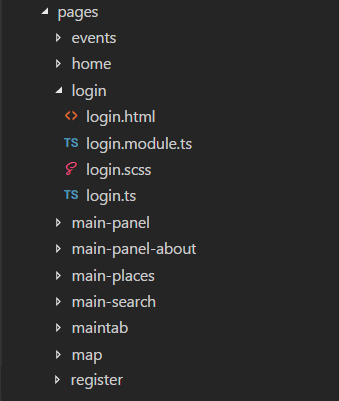
\includegraphics[
   keepaspectratio=true
]{./06_Implementacion/img/estructuraionicsrcpages.png}
\caption{Estructura aplicación \textit{Ionic - pages}}
\end{figure}

Para cada \textit{page} tenemos:
\begin{itemize}
	\item Un archivo HTML que contiene la vista de la página.
	\item Un archivo SCSS que contiene los estilos de la vista.
	\item Dos archivo TypeScript. Uno que actúa de controlador y otro que sirve para la configuración de las vistas.
\end{itemize}



\section{Implementación capa modelo}

\subsection{Persistencia}
Para la implementación de la persistencia de la aplicación se han seguido las definiciones especificadas en la API de persistencia para la plataforma Java, conocida comúnmente como JPA. Esta API nos proporciona una gestión de los datos relacionales en nuestra aplicación Java.


Puesto que JPA solo define un conjunto de interfaces, es necesaria una implementación de las mismas, que en este caso, será gracias al framework de Hibernate. Hibernate no solo implementa las especificaciones de JPA sino que también incorpora funcionalidades propias.


\subsubsection*{Implementación clases persistentes}
A continuación se mostrará un ejemplo de una entidad con las anotaciones definidas por JPA.

\begin{figure}[H]
\centering
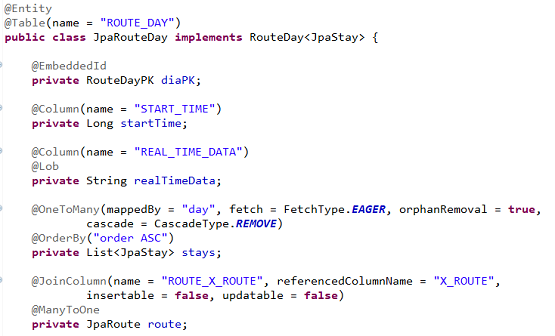
\includegraphics[
   keepaspectratio=true
]{./06_Implementacion/img/implclasespersist.png}
\caption{Implementación clases persistentes}
\end{figure}

A continuación se explican, brevemente, las anotaciones JPA empleadas.

\begin{itemize}
	\item \textbf{@Entity. }Declara una clase POJO como entidad persistente. 
	\item \textbf{@Table. }Especifica la tabla empleada para la clase marcada como @Entity. 
	\item \textbf{@EmbeddedId. }Denota una clave primaria compuesta que es una clase marcada por @Embeddable. Se aplica sobre un campo o propiedad persistente de la clase.
	\item \textbf{@Column. }Anotación utilizada para \textit{mapear} una columna con la propiedad o campo de la clase. El atributo \textit{name} permite especificar el nombre de la columna.
	\item \textbf{@Lob. } Determina que la propiedad debe persistir como una estructura que permita almacenar gran cantidad de información.
	\item \textbf{@OneToMany. }Define una relación de uno a muchos entre dos entidades. 
	\item \textbf{@OrderBy. }Especifica el orden de los elementos de la colección cuando son recuperados.
	\item \textbf{@JoinColumn. }Determina una columna para unir una entidad de asociación.
	\item \textbf{@ManyToOne. }Define una relación muchos a uno.
\end{itemize}



\subsubsection*{Implementación DAOs}
Como se ha comentado en el apartado de \textit{Diseño}, se ha elaborado un DAO genérico que implementa un conjunto de funcionalidades básicas. Para las consultas a la base de datos, realizadas por el DAO, se ha utilizado \textit{JPA Criteria API}, que nos permite definir las consultas para las entidades mediante la creación de una serie de objetos. A continuación, se muestra un ejemplo de uso de esta API.

\begin{figure}[H]
\centering
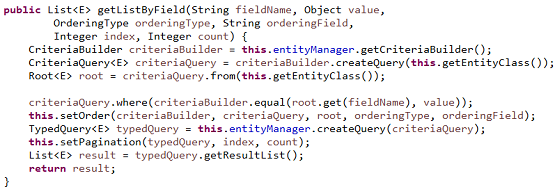
\includegraphics[
   keepaspectratio=true
]{./06_Implementacion/img/impldao.png}
\caption{Implementación consultas DAO}
\end{figure}

En este ejemplo, se define el método \textit{getListByField(...)} que nos devolverá la lista de objetos que cumplan filtro aplicado. Como se puede observar en la imagen, la consulta a la base de datos se ha realizado mediante la utilización de las clases ofrecidas por la API de Criteria.


\subsubsection*{Gestión de la transaccionalidad}
La lógica de negocio de la aplicación hace uso de los DAOs creados anteriormente y que realizan diferentes operaciones sobre la base de datos. Debido a que en un mismo caso de uso pueden realizar diferentes operaciones de los DAOs, es necesario crear una transacción que nos permita ejecutar todas esas acciones contra la base de datos en bloque y que, en caso de que alguna produjese un error, poder deshacer los cambios ocasionados por las demás.

Para ello, será necesario anotar estos métodos con la anotación \textit{@Transactional}. Con esta anotación, se empezará una transacción antes de la primera línea del método y que terminará justo después de la última, permitiendo ejecutar todo lo que esté dentro del método dentro de una misma transacción.

\begin{figure}[H]
\centering
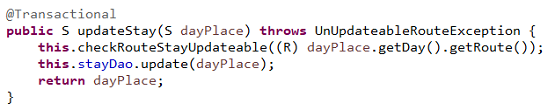
\includegraphics[
   keepaspectratio=true
]{./06_Implementacion/img/impltransactional.png}
\caption{Implementación ejemplo transaccionalidad}
\end{figure}

En la figura 7.17, se define el método \textit{updateStay} marcado con la anotación comentada anteriormente, de forma que, todas las operaciones ejecutadas dentro del método se encontrarán dentro de una misma transacción. 


\section{Implementación capa servicios}
La aplicación está formada por una serie de servicios web REST que ofrecen las funcionalidades de la capa modelo remotamente. Como se había comenta, estos servicios han sido elaborados siguiendo las especificaciones establecidas por la API JAX-RS.

A continuación, se muestra un ejemplo de un recurso web, donde se explica, brevemente, la función de cada anotación.


\begin{figure}[H]
\centering
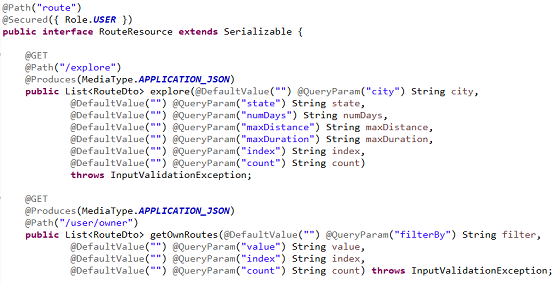
\includegraphics[
   keepaspectratio=true
]{./06_Implementacion/img/implapirest.png}
\caption{Implementación ejemplo transaccionalidad}
\end{figure}

\begin{itemize}
	\item \textbf{@Path. }Identifica la URI en la que responderá un o método o recurso de la clase. Toma un valor relativo, siendo la URI base el \textit{path} de la aplicación.
	\item \textbf{@Secured. }Anotación personalizada. Creada para marcar el recurso como seguro de manera que se aplica un filtro de autenticación para cada petición.
	\item \textbf{@GET. }Indica que el método anotado responde a solicitudes HTTP GET.
	\item \textbf{@Produces. }Define el \textit{mediatype} que pueden generar los métodos. Análogamente, existe la anotación @Consumes, que define el \textit{mediatype} que acepta el método.
	\item \textbf{@QueryParam. }Vincula el valor del parámetro HTTP a un parámetro del método.
	\item \textbf{@DefaultValue. }Especifica un valor predeterminado para la anotación @QueryParam.
\end{itemize}



\section{Implementación autenticación y autorización}


\section{Implementación cliente web}


\section{Implementación cliente móvil}
